% !TeX root = main.tex
\documentclass[11pt,a4paper]{article}

% \documentclass[a4paper,14pt, draft]{article}

%%% отключение нумерации сраниц
\pagestyle{empty}
%%% значок в itemize
% \renewcommand{\labelitemi}{$\cdot$}

%%% Работа с русским языком
\usepackage{cmap}					% поиск в PDF
\usepackage{mathtext} 				% русские буквы в формулах
\usepackage[T1, T2A]{fontenc}			% кодировка %Т1 посоветовал чат гпт
\usepackage[utf8]{inputenc}			% кодировка исходного текста
\usepackage[english,russian]{babel}	% локализация и переносы
\usepackage{indentfirst}            % красная строка в первом абзаце
\frenchspacing                      % равные пробелы между словами и предложениями

%%% Дополнительная работа с математикой
\usepackage{amsmath,amsfonts,amssymb,amsthm,mathtools} % пакеты AMS
\usepackage{icomma}                                    % "Умная" запятая

%%% Свои символы и команды
\usepackage{centernot} % центрированное зачеркивание символа
\usepackage{stmaryrd}  % некоторые спецсимволы
\usepackage{dsfont}
\usepackage{amsthm}


\renewcommand{\epsilon}{\ensuremath{\varepsilon}}
\renewcommand{\phi}{\ensuremath{\varphi}}
\renewcommand{\kappa}{\ensuremath{\varkappa}}
\renewcommand{\le}{\ensuremath{\leqslant}}
\renewcommand{\leq}{\ensuremath{\leqslant}}
\renewcommand{\ge}{\ensuremath{\geqslant}}
\renewcommand{\geq}{\ensuremath{\geqslant}}
\renewcommand{\emptyset}{\ensuremath{\varnothing}}

\DeclareMathOperator{\sgn}{sgn}
\DeclareMathOperator{\ke}{Ker}
\DeclareMathOperator{\im}{Im}
\DeclareMathOperator{\re}{Re}

\newcommand{\N}{\mathbb{N}}
\newcommand{\Z}{\mathbb{Z}}
\newcommand{\Q}{\mathbb{Q}}
\newcommand{\R}{\mathbb{R}}
\newcommand{\Cm}{\mathbb{C}}
\newcommand{\F}{\mathbb{F}}
\newcommand{\id}{\mathrm{id}}
\newcommand{\imp}[2]{
	(#1\,\,$\ra$\,\,#2)\,\,
}
\newcommand{\Root}[2]{
	\left\{\!\sqrt[#1]{#2}\right\}
}
\newcommand{\RR}{\R}
\newcommand{\NN}{\N}
\renewcommand{\subseteq}{\subset}
\newcommand{\sub}{\subset}
\newcommand{\sconstr}{\;\vert\;}
\newcommand{\thus}{\implies}

\newcommand{\defeq}{\vcentcolon= }
\newcommand{\defev}{\stackrel{\Delta}{\Longleftrightarrow}}
\newcommand{\deriv}[3][1]{%
	\ifthenelse{#1>1}{%
		\frac{\dlta^{#1} {#2}}{\dlta {#3}^{#1}}
	}{%
		\frac{\dlta {#2}}{\dlta {#3}}
	}%
}

\renewcommand\labelitemi{$\triangleright$}

\let\bs\backslash
\let\lra\Leftrightarrow
\let\ra\Rightarrow
\let\la\Leftarrow
\let\emb\hookrightarrow

%%% Перенос знаков в формулах (по Львовскому)
\newcommand{\hm}[1]{#1\nobreak\discretionary{}{\hbox{$\mathsurround=0pt #1$}}{}}

%%% Работа с картинками
\usepackage{graphicx}    % Для вставки рисунков
\setlength\fboxsep{3pt}  % Отступ рамки \fbox{} от рисунка
\setlength\fboxrule{1pt} % Толщина линий рамки \fbox{}
\usepackage{wrapfig}     % Обтекание рисунков текстом

% \usepackage[inkscapeformat=png]{svg} %% svg

%%% Работа с таблицами
\usepackage{array,tabularx,tabulary,booktabs} % Дополнительная работа с таблицами
\usepackage{longtable}                        % Длинные таблицы
\usepackage{multirow}                         % Слияние строк в таблице

%%% Теоремы
\theoremstyle{plain}
\newtheorem*{theorem}{Теорема}
\newtheorem*{lemma}{Лемма}
\newtheorem*{proposition}{Утверждение}
\newtheorem*{exercise}{Упражнение}
\newtheorem*{problem}{Задача}

\theoremstyle{definition}
\newtheorem*{definition}{Определение}
\newtheorem*{corollary}{Следствие}
\newtheorem*{note}{Замечание}
\newtheorem*{reminder}{Напоминание}
\newtheorem*{example}{Пример}

\theoremstyle{remark}
\newtheorem*{solution}{Решение}

%%% Оформление страницы
\usepackage{extsizes}     % Возможность сделать 14-й шрифт
\usepackage{geometry}     % Простой способ задавать поля
\usepackage{setspace}     % Интерлиньяж
\usepackage{enumitem}     % Настройка окружений itemize и enumerate
\setlist{leftmargin=10pt} % Отступы в itemize и enumerate

\geometry{top=15mm}    % Поля сверху страницы
\geometry{bottom=5mm} % Поля снизу страницы
\geometry{left=10mm}   % Поля слева страницы
\geometry{right=10mm}  % Поля справа страницы

\setlength\parindent{15pt}        % Устанавливает длину красной строки 15pt
\linespread{1}                  % Коэффициент межстрочного интервала
%\setlength{\parskip}{0.5em}      % Вертикальный интервал между абзацами
\setcounter{secnumdepth}{0}      % Отключение нумерации разделов
%\setcounter{section}{-1}         % Нумерация секций с нуля
\usepackage{multicol}			  % Для текста в нескольких колонках
\usepackage{soulutf8}             % Модификаторы начертания
\mathtoolsset{showonlyrefs=true} % показывать номера формул только у тех, у которых есть ссылки по eqref
%%% Содержаниие
% \usepackage{tocloft}
% \tocloftpagestyle{main}
%\setlength{\cftsecnumwidth}{2.3em}
%\renewcommand{\cftsecdotsep}{1}
%\renewcommand{\cftsecpresnum}{\hfill}
%\renewcommand{\cftsecaftersnum}{\quad}

%%% Нумерация уравнений
\makeatletter
\def\eqref{\@ifstar\@eqref\@@eqref}
\def\@eqref#1{\textup{\tagform@{\ref*{#1}}}}
\def\@@eqref#1{\textup{\tagform@{\ref{#1}}}}
\makeatother                      % \eqref* без гиперссылки
\numberwithin{equation}{section}  % Нумерация вида (номер_секции).(номер_уравнения)
\mathtoolsset{showonlyrefs= true} % Номера только у формул с \eqref{} в тексте.

%%% Гиперссылки
\usepackage{hyperref}
\usepackage[usenames,dvipsnames,svgnames,table,rgb]{xcolor}
\hypersetup{
	unicode=true,            % русские буквы в раздела PDF
	colorlinks=true,       	 % Цветные ссылки вместо ссылок в рамках
	linkcolor=black!15!blue, % Внутренние ссылки
	citecolor=green,         % Ссылки на библиографию
	filecolor=magenta,       % Ссылки на файлы
	urlcolor=NavyBlue,       % Ссылки на URL
}

%%% Графика
\usepackage{tikz}        % Графический пакет tikz
\usepackage{tikz-cd}     % Коммутативные диаграммы
\usepackage{tkz-euclide} % Геометрия
\usepackage{stackengine} % Многострочные тексты в картинках
\usetikzlibrary{angles, babel, quotes}
% \title{$\mathbb{O} \mathbb{B} \mathbb{A} \mathbb{T} $и$ \mathbb{K}$}
\title{\texttt{2.1.3 Определение $C_p /C_v$ по скорости звука в газе}}\date{}\author{}
\begin{document}
\maketitle
  \textbf{Цель работы:} $1)$ измерение частоты колебаний и длины волны при
  резонансе звуковых колебаний в газе, заполняющем трубу; $2$) опреде-
  ление показателя адиабаты с помощью уравнения состояния идеаль-
  ного газа.\\
  \textbf{В работе используется:} Звуковой генератор ГЗ; электронный ос-
  циллограф ЭО; микрофон; телефон; раздвижная труба; теплоизоли-
  рованная труба, обогреваемая водой из термостата; баллон со сжатым
  углекислым газом; газгольдер.

\section*{Теория}
  Скорость звука в газах: 
  \begin{equation*}
    c = \sqrt{\gamma\frac{RT}{\mu}}
  \end{equation*}
  $\gamma$ -- показатель адиабаты.
  Тогда:
  \begin{equation*}
    \gamma = \frac{\mu}{RT}c^2
  \end{equation*}
  $f$ -- частота звука, $\lambda$ -- длина волны, тогда:
  \begin{equation*}
    c = \lambda f
  \end{equation*}
  Чтобы возникали стоячие волны (резонансы), должно выполняться:
  \begin{equation*}
    L = n\frac{\lambda}{2}
  \end{equation*}
  Для k-ой гармоники (относительно самого низкой частоты, при которой возникает стоячая волна):
  \begin{equation*}
    f_k= = f_1 + \frac{c}{2L} \cdot (k - 1)
  \end{equation*}

\section*{Экспериментальная установка}
  Микрофон и телефон присоединены к установке через тонкие резиновые трубки. 
  Такая связь достаточна для возбуждения и обнаружения звуковых колебаний 
  в трубе и в то же время мало возмущает эти колебания: при расчётах оба торца трубы можно считать неподвижными, а
  влиянием соединительных отверстий пренебречь.
  \begin{figure}[h]
    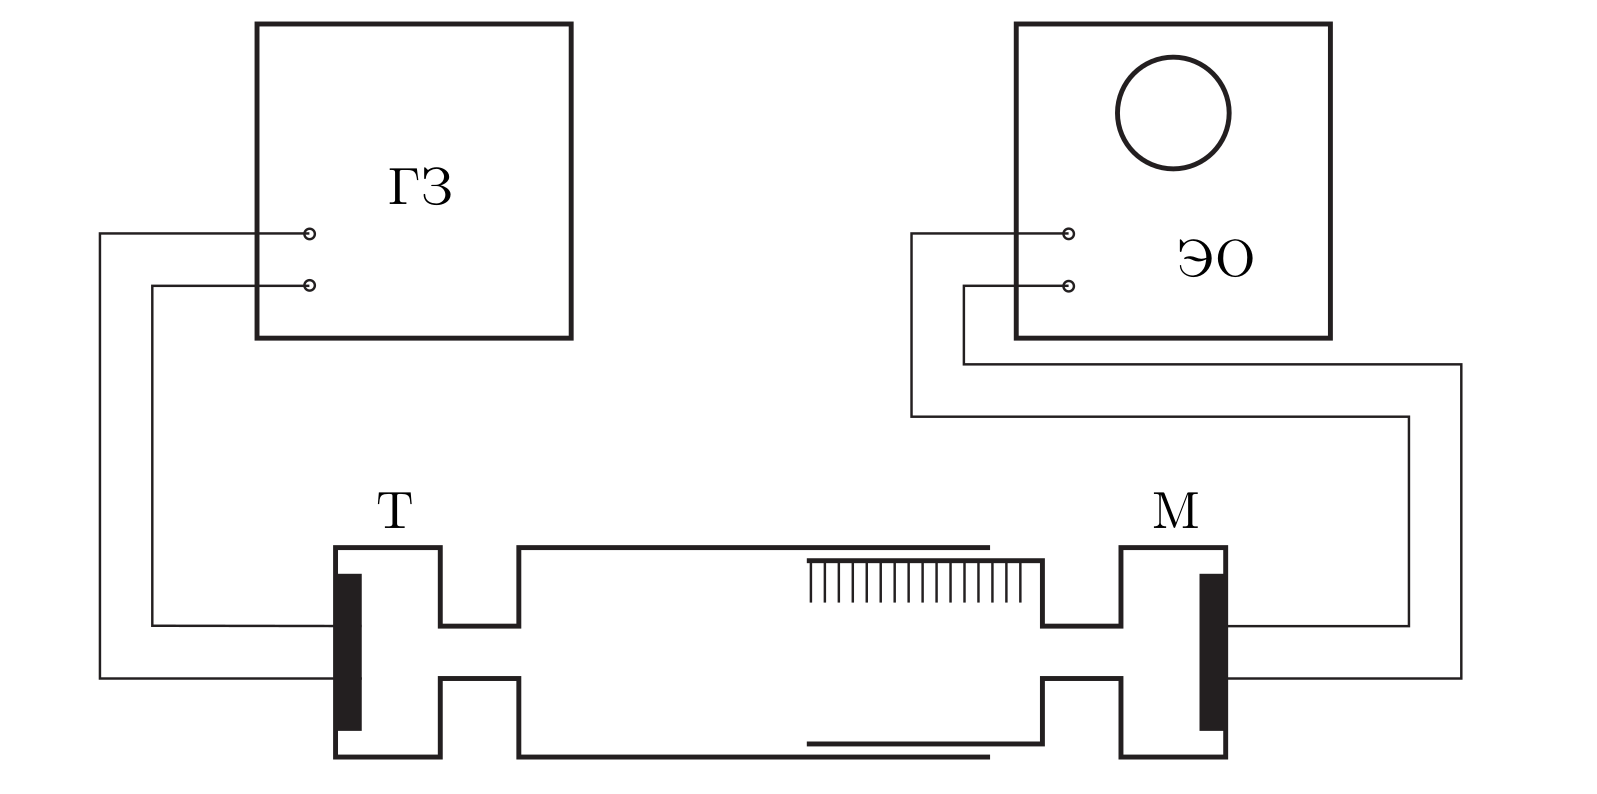
\includegraphics[width=\textwidth]{movingtube.png}
    \caption{Установка для измерения скорости звука
    при помощи раздвижной трубы}
  \end{figure}
  \begin{figure}[h]
    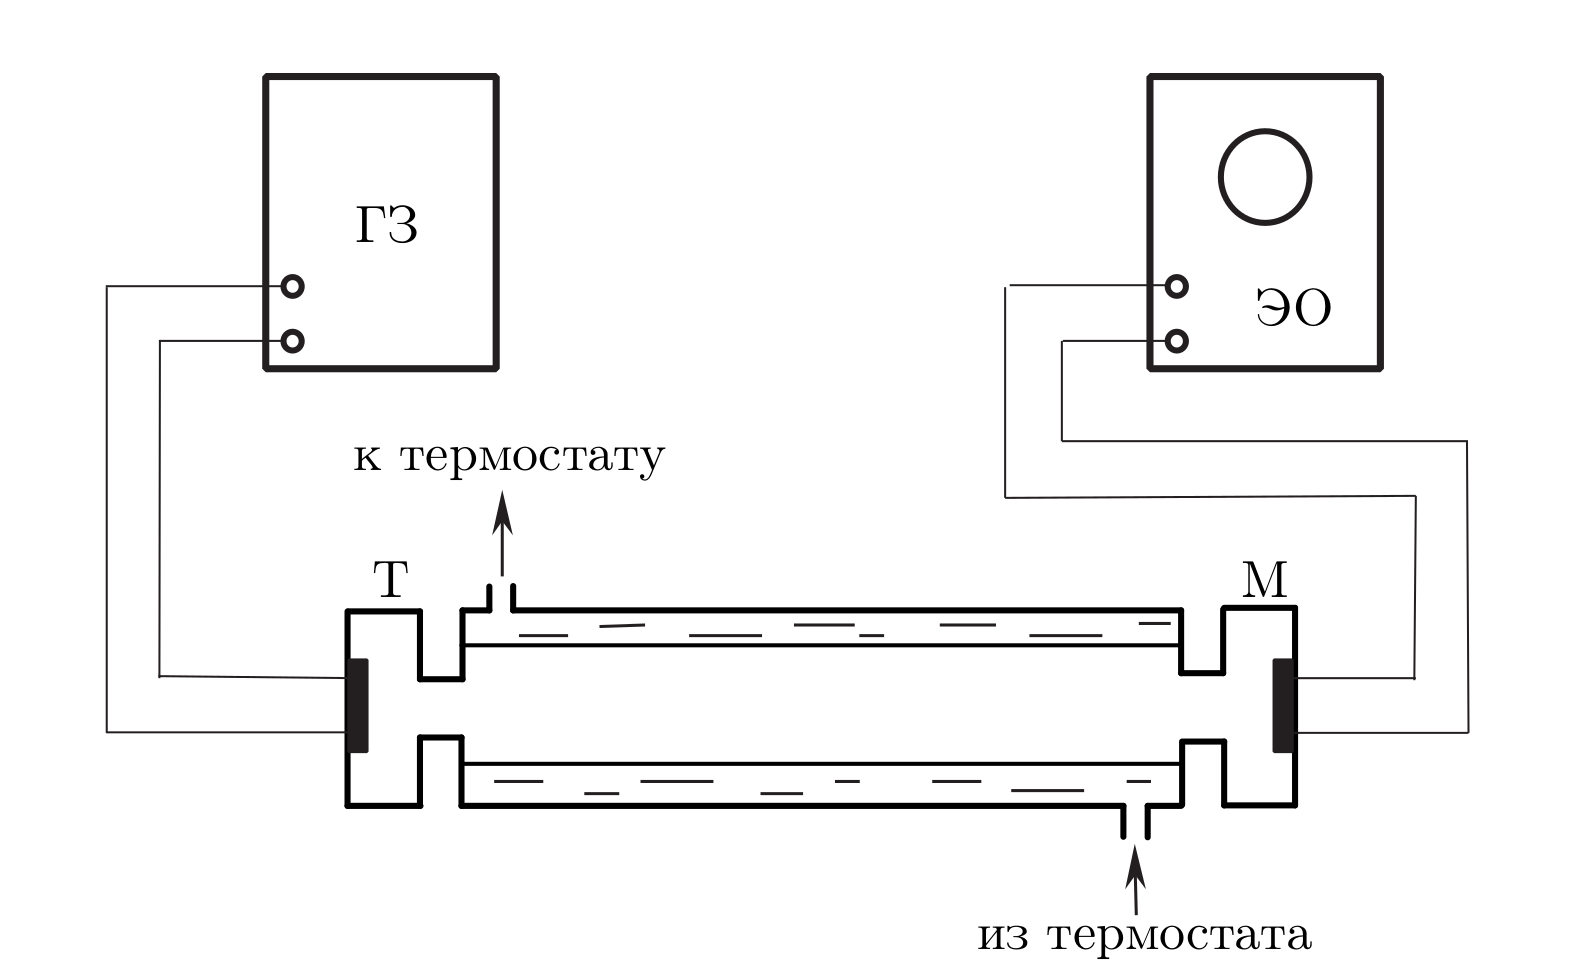
\includegraphics[width=\textwidth]{c ot t.png}
    \caption{Установка для изучения зависимости скорости звука
    от температуры}
    \label{lala}
  \end{figure}
  Первая установка (Рис. 1) содержит раздвижную трубу с миллиметровой шкалой. 
  Через патрубок (на рисунке не показан) труба может наполняться воздухом 
  или углекислым газом из газгольдера. На
  этой установке производятся измерения $\gamma$ для воздуха и для $CO_2$ . 
  Вторая установка (Рис. 2) содержит теплоизолированную трубу постоянной
  длины. Воздух в трубе нагревается водой из термостата. Температура
  газа принимается равной температуре воды, омывающей трубу. На этой
  установке измеряется зависимость скорости звука от температуры.

\section*{Ход эксперимента}
figure~\pageref{lala}
\end{document}